\section*{Implementation Plan}

We plan to adapt the vision system presented by Sharp, Shakernia, and Sastry in
their 2001 paper, ``A Vision System for Landing an Unmanned Aerial Vehicle''.
Their system continuously estimates the camera's pose with respect to the
landing platform, if it is within visual range. They use several techniques we
studied in CS280, such as corner detection and structure-from-motion. We will
evaluate our vision algorithm by comparing its pose estimate with the
quadcopter's internal pose estimate (which is based on GPS and inertial
sensors), and also by performing test landings. Figure \ref{fig:platform} shows
the prototype landing station we have built for testing our algorithm.

\begin{figure}[h!]
    \centering
    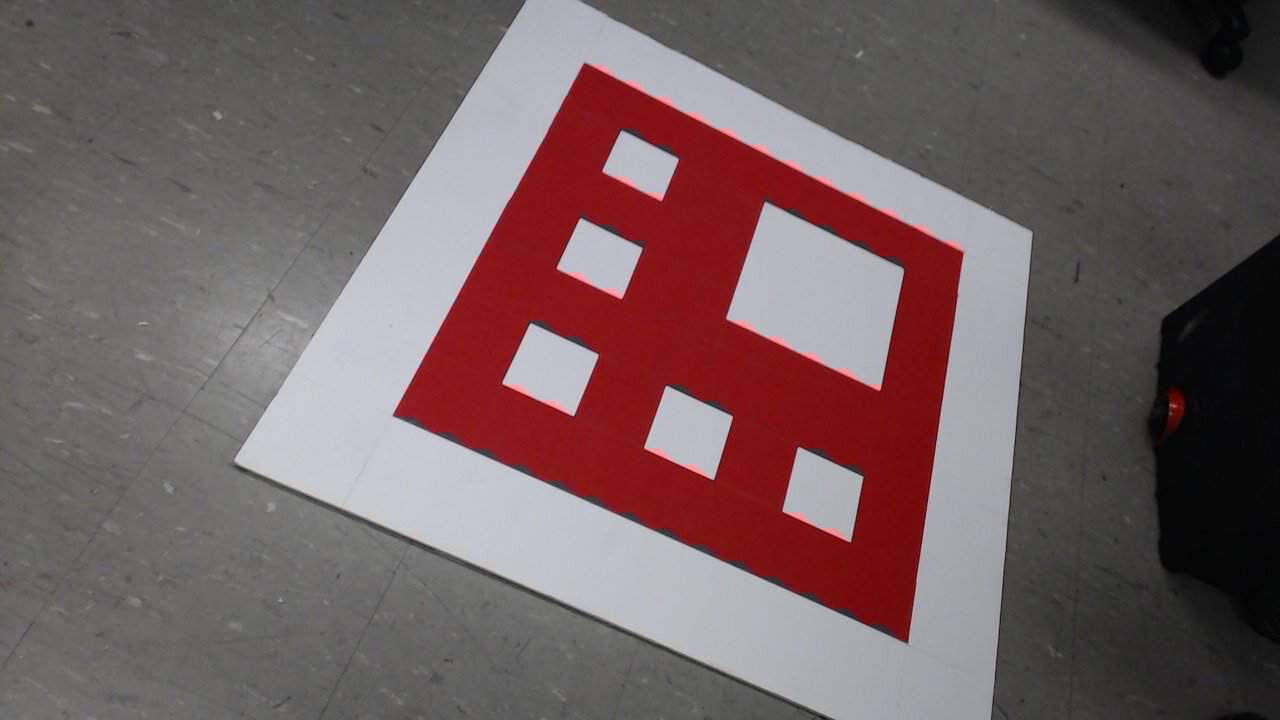
\includegraphics[width=0.5\textwidth]{platform.jpg}
    \caption{Prototype landing platform seen from an angle}
    \label{fig:platform}
\end{figure}
